%**************************************************************
\chapter{Pagine interne}
\label{cap:pagine-interne}
%**************************************************************
Navigando nel sito si può notare come non ci sia una gerarchia tra le pagine, e non ci sia un'alberatura profonda quindi è difficile che l'utente "si perda" navigando nel sito. Di conseguenza l'uso di un breadcrumb sarebbe stato del tutto inutile. Tuttavia è bene ogni pagina interna rispetti gli assi obbligatori who e what.
\begin{figure}[ht]
    \centering
    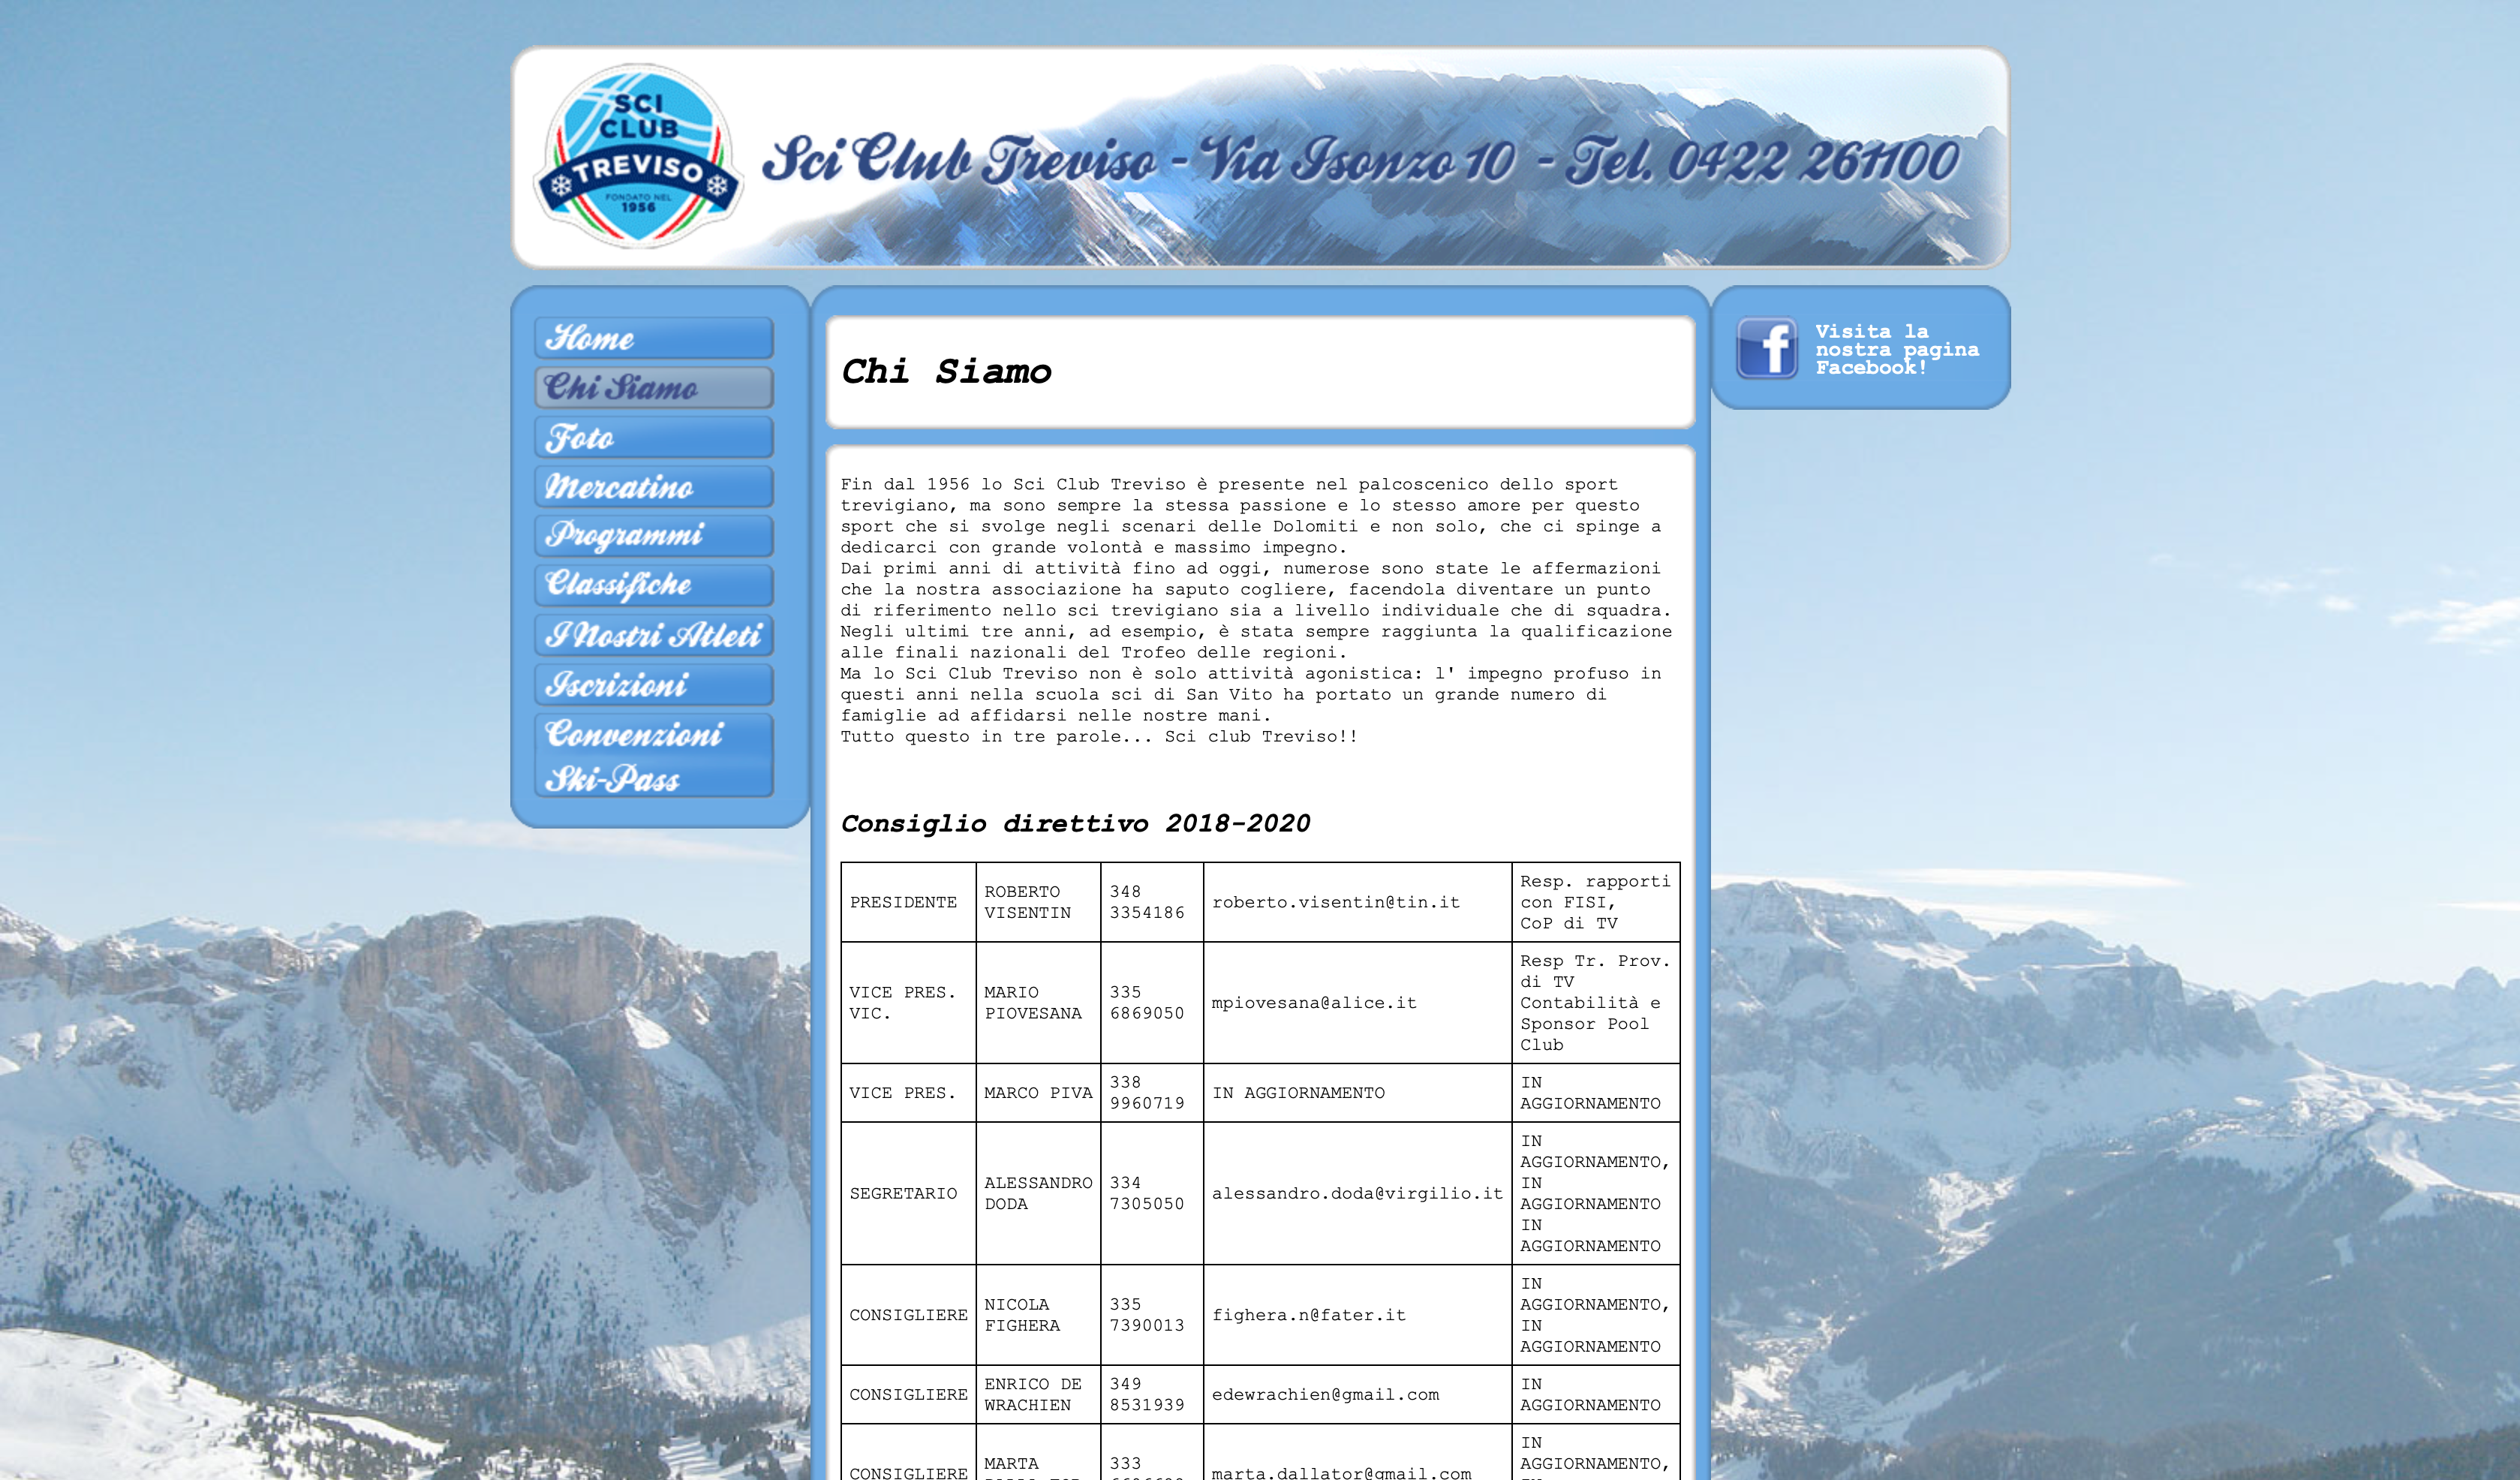
\includegraphics[scale=0.2]{./immagini/chi-siamo}
    \caption [Pagina Chi Siamo]{Pagina Chi Siamo}
\end{figure}

Ogni pagina interna è identificata da un titoletto, lo stesso presente nel menù a sinistra, che consente all'utente di sapere in che pagina si trova. Inoltre, al click di una voce di menù, questa cambia di colore offrendo un'informazione aggiuntiva sulla pagina che si sta visitando.